\documentclass{ieeeaccess}
\usepackage{amsmath,amssymb,amsfonts}
\usepackage{graphicx}
\usepackage{textcomp}

\usepackage{bm}
\makeatletter
\AtBeginDocument{\DeclareMathVersion{bold}
\SetSymbolFont{operators}{bold}{T1}{times}{b}{n}
\SetSymbolFont{NewLetters}{bold}{T1}{times}{b}{it}
\SetMathAlphabet{\mathrm}{bold}{T1}{times}{b}{n}
\SetMathAlphabet{\mathit}{bold}{T1}{times}{b}{it}
\SetMathAlphabet{\mathbf}{bold}{T1}{times}{b}{n}
\SetMathAlphabet{\mathtt}{bold}{OT1}{pcr}{b}{n}
\SetSymbolFont{symbols}{bold}{OMS}{cmsy}{b}{n}
\renewcommand\boldmath{\@nomath\boldmath\mathversion{bold}}}
\makeatother

\def\BibTeX{{\rm B\kern-.05em{\sc i\kern-.025em b}\kern-.08em
    T\kern-.1667em\lower.7ex\hbox{E}\kern-.125emX}}

\usepackage{tabularx}
\usepackage[hidelinks]{hyperref}
\usepackage{etoolbox}
\usepackage{multicol}
\hypersetup{pdftitle={Swapping Initial Motor Temperatures Changes Route Feasibility for a Simulated Hexapod},
  pdfsubject={IEEE Access manuscript on hot-motor swaps}, pdfkeywords={hexapod, simulation, thermal management}}
\makeatletter
% Hide the DOI label until the journal assigns a DOI.
\patchcmd{\@maketitle}
  {{\vss\doifont Digital Object Identifier\space\@doi\vss}\vspace*{7.4mm}\par}
  {\ifx\@doi\@empty\else
     {\vss\doifont Digital Object Identifier\space\@doi\vss}\vspace*{7.4mm}\par
   \fi}
  {}{\PackageError{manuscript}{Could not adjust the DOI line}{}}
% Keep page numbers and suppress the volume label until assignment.
\newcommand{\accessVolumeFooter}{%
  \ifx\thevol\@empty\else\footervolfont VOLUME\ \thevol, \theyear\fi}
\newcommand{\adjustAccessVolumeFooter}[1]{%
  \patchcmd{#1}{\footervolfont VOLUME\ \thevol, \theyear}{\accessVolumeFooter}{}{}%
  \patchcmd{#1}{\footervolfont VOLUME\ \thevol, \theyear}{\accessVolumeFooter}{}{}}
\adjustAccessVolumeFooter{\ps@titlepage}
\adjustAccessVolumeFooter{\ps@headings}
\pagestyle{headings}
\makeatother
\AtBeginDocument{%
  \patchcmd{\thebibliography}
    {\addcontentsline{toc}{section}{\refname}}
    {\phantomsection\addcontentsline{toc}{section}{\refname}}
    {}{}%
}
\makeatletter
% Keep each appendix display and its caption together at its source position.
\newenvironment{appendixdisplay}[1]
  {\par\addvspace{4pt}\noindent\begin{minipage}{\linewidth}\def\@captype{#1}}
  {\end{minipage}\par\addvspace{6pt}}
\makeatother
\setlength{\multicolsep}{5pt}
\begin{document}
% Replace the review placeholders with the confirmed author list and affiliations.
\history{Version 3 review draft for author verification.}
\doi{Pending assignment}
\vol{-}
\year{-}

\author{\uppercase{Author information pending}\authorrefmark{1}}
\address[1]{Affiliation pending author confirmation}
\corresp{Corresponding author information pending confirmation.}
% Add verified funding information with \tfootnote{...} when applicable.
\markboth{Version 3 review draft: Hot-Motor Swaps and Hexapod Routing}{Version 3 review draft: Hot-Motor Swaps and Hexapod Routing}

\title{Swapping Initial Motor Temperatures Changes Route Feasibility for a Simulated Hexapod}
\begin{abstract}
We examined if changing the order of onset of warm starts/warms results in a change of the equivalent sets of routes that can be completed by a hexapod with a fixed average and maximum starting temperature. For the MuJoCo experiment, the four paths were set on 12 two-stage courses, with three temperature settings. We tried all 4 routes on both warm side assignments and got 288 walks in a row, for 72 starts. In 11 of the 36 course--setting pairs, each assignment had at least one finishable route and no route finished under both assignments. We compared a planner that received individual motor temperatures with a planner that received their mean and maximum and averaged forecasts over the two possible assignments. Both used the same temperature-responsive speed controller with individual motor temperatures during walking. The per-motor planner finished 26 of 72 starts and recorded two thermal stops. The aggregate planner ended up 7-72 and had five thermal stops. The gain was 26.4 percentage points with a descriptive 95\% course-re-sample interval of 15.3-40.3 percentage points. These exhaustive replays illustrate the variability of the route's feasibility or completion as a result of varying initial heat distributions across motors when simulated under the tested conditions.
\end{abstract}

\begin{keywords}
Actuator temperature, hexapod robots, legged locomotion, path planning, thermal management
\end{keywords}
\titlepgskip=-21pt
\maketitle

\section{Introduction}

\PARstart{A}{} robot that starts with a few warm motors will have less thermal head room. Routes can have several legs, particularly on banks that have different inclines. The warm values may be attached to various legs, but be the same for two starting states. We ask ourselves whether a change in this alone changes which full-routes to the goal can be made without over heating.

To answer this question, we test this scenario in simulation; every route is replayed with the same nine warm and nine cool temperatures except that each is assigned to opposite sides of the hexapod. A version of Trujillo and Cutkosky's controller \cite{trujillo2009} is used to have the robot continually pass through a junction, modifying its speed according to the temperatures of its motors. The route replays establish which routes finish in each starting state, including routes that the planners reject. A separate matched comparison compares the benefits of using the entire temperature assignment (or solution) to select a route. The execution controller is shared between both arms and the two arms differ in the initial temperature information used to select a route.

The main finding is the number of times both starting states are finishable and the number of different routes that are required to finish both states. Planner comparison makes comparisons on on-time completion and thermal stops for like starts. A previous matched experiment explored the impact on completion of planning a \textquotedbl{}cooling pause\textquotedbl{} at an intersection. We present that experiment separately in Appendix~\ref{app:pause}.

\section{Related Work}

\subsection{Thermal Modeling And Control}

Lumped thermal models predict temperature transients in electrical machines \cite{mellor1991}. De et al. added the consideration of motor thermal dynamics in addition to the timing of a representative task to actuator sizing of legged robots \cite{de2011}. Lin et al. identified a coupled thermal network for a quadruped that incorporates heat exchange between components and forced convection during locomotion \cite{lin2025}. In our simulation, each actuator's temperature evolves independently according to its applied torque history and the cooling term.

Using a motor thermal constraint \cite{trujillo2009} a controller was implemented by Trujillo and Cutkosky to regulate climbing speed. Tan et al. included temperature limits in robot trajectory optimization, and Kawaharazuka et al. estimated and controlled motor core temperature while updating model parameters online \cite{tan2018heat}, \cite{kawaharazuka2020}. Temperature constraints have also been imposed on motor drivers in predictive control for a redundant manipulator \cite{debenedittis2026}. Two recent quadruped preprints address thermal limits at the locomotion-policy level. Wan et al. conditioned a residual policy on motor thermal state, and Ségas et al. trained a policy to reduce the highest predicted steady-state motor temperatures \cite{wan2026}, \cite{segas2026}.

Faigl and \v{C}\'{\i}\v{z}ek measured servo temperatures during uneven-terrain trials with a hexapod and used standing breaks for cooling \cite{faigl2019}. Brodoline et al. measured power use in a static pose on a servomotor leg test bench \cite{brodoline2024}. Jorgensen et al. optimized contact-constrained postures to reduce predicted actuator temperatures and demonstrated the approach on Valkyrie \cite{jorgensen2019}. Urata and Ito described predicting individual motor temperatures during continued walking and during a transition to a standing cooling posture \cite{urata2017}.

\subsection{Terrain, Contact Loads, And Energy}

Hexapod studies have used joint torque and inertial measurements to adapt compliance to terrain, and optimized contact-force distribution during walking on rugged terrain \cite{zhao2021}, \cite{ding2024}. For quadrupeds on slopes, Gehring et al. adapted locomotion to estimated inclination, and Focchi et al. optimized contact forces to limit actuator effort while satisfying friction constraints \cite{gehring2015}, \cite{focchi2017}. Righetti et al. showed how contact-force objectives can be incorporated into floating-base robot control \cite{righetti2013}. Inspired by these studies, in the simulation actuator effort is tracked on each branch.

Hexapod locomotion has been studied in terms of the swing trajectories over irregular surfaces \cite{luneckas2019} and gait selection based energy use and COT \cite{luneckas2021}. When characterizing energy use in the MIT Cheetah \cite{seok2015}, Seok et al. have taken into consideration motor heat loss. In order to improve the efficiency and robustness of step placement and timing parameters, they were optimized by Schperberg et al. \cite{schperberg2025}. Predicted arrival time and peak motor temperature are what we have in our route screen.

\subsection{Terrain-Aware Locomotion Planning}

Contact planning on different terrains has been a combination of the planning of discrete stance or contact sequence plus continuous motion planning \cite{hauser2008} \cite{valouch2021}. Jenelten et al. optimized footholds from onboard elevation maps, while Mastalli et al. jointly planned body motion, footholds, and step durations with terrain costs \cite{jenelten2020}, \cite{mastalli2020}. Brandão et al. optimized a mechanical work model for humanoid footsteps subject to feasibility and ground friction constraints on slanted and slippery terrain \cite{brandao2016}.

At route scale, Prágr et al. learned gait-specific traversability models for hexapod exploration and used them to choose navigation waypoints \cite{pragr2022}. Fu et al. coupled global path planning with proprioceptive information from the walking robot, and Yang et al. planned routes for a quadruped using learned motion costs that included energy, time, and risk \cite{fu2022}, \cite{yang2021}. David et al. adjusted navigation costs using the robot's internal hazard state under environmental heat and radiation exposure \cite{david2022}. In our study, initial temperature values are set to fixed values and their distributions to motors are changed. Checks exhaustively which routes can be completed at each assignment as the speed controller responds to the temperature.

\newpage
\section{Methods}

\subsection{Course Network And Execution Outcomes}
\label{subsec:routing}

With every course there is a start, a flat junction and a goal. There are 4 branches: 2 branches with the start and 2 branches with the goal. Each of the four routes is specified by its branch number in the first stage and its branch number in the second stage. Each replay follows the specified route in one continuous run. The chassis, foot, controller, and motor states carry through the junction.

\begin{figure}[!b]
\centering
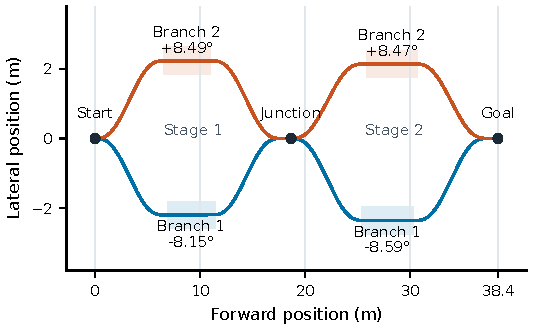
\includegraphics[width=\columnwidth]{figures/swap_course.pdf}
\caption{Top view of persistent-bank course P3. Each stage has two branch centerlines. The centerlines meet at the flat junction. The four routes are the combinations of the two branch choices in each stage.}
\label{fig:graph}
\end{figure}

Here is one of the 12 synthetic heightfields (shown in Fig.~\ref{fig:graph}). Smooth approach and exit curves connect the common landings to each branch. The bank fades in and out along the branch and tapers laterally. The courses vary the approach and exit lengths, bank lengths, lateral offsets, bank angles, and longitudinal bank shifts. There are four alternating-bank courses (A1--A4) whose signs reverse across stages on each branch, four persistent-bank courses (P1--P4) whose signs persist, and four courses (S1--S4) with a stage in which both branches bank in the same direction. Geometry and deadlines were determined prior to nominal and warm replays. The geometry is given in Appendix~\ref{app:course-data}.

The intended grid size of the heightfield was 0.12 m. The estimates were 38.03--39.56 m forward. The end time for each course was based on the length of the course / 0.108 m/s and rounded to the nearest whole second, which resulted in a projected end time of 352 to 366 s. The rate kept the same benchmark from before, with a section of a scale that indicates the timeframe for the deadline. The planner deadlines were the same for both warm-side assignments and both planners. Arrival meant that the chassis had to get into the 0.55 m radius around the goal. We checked the lateral error from the route centerline at the same forward coordinate and used a limit of 0.85 m. The initial stand counts toward the deadline.

A completion required arrival within the deadline without a fall, chassis contact, corridor departure, or thermal stop. The simulator stops a run at the first recorded sample at which any motor reaches $T_{\mathrm{lim}}=70\,{}^\circ\mathrm{C}$. It checks this condition before checking arrival in the same sample. The planners use a forecast cutoff of $T_{\mathrm{cap}}=T_{\mathrm{lim}}-0.50\,{}^\circ\mathrm{C}$.

\subsection{Hexapod And Physics Execution}

The simulation used MuJoCo 3.9.0 \cite{todorov2012}. The hexapod had a floating chassis and three torque-actuated joints per leg at the coxa, femur, and tibia. The simplified geometry was informed by the computer-aided design (CAD) assembly and had a modeled total mass of 82 kg, including the feet. From proximal to distal, the segment lengths were 0.157, 0.550, and 0.740 m, and the nominal joint torque limits were 90, 150, and 130 $\mathrm{N}{\cdot}\mathrm{m}$. A 3 s crawl gait generated foot targets from the branch centerline and simulated terrain height. Joint position and velocity feedback generated tracking torque. The desired chassis force and moment were allocated by a regularized least-squares allocation for the supporting feet. The time of the physics step was in 2 ms. Body positions and the number of contacts were reported by the simulator and the thermal model (60 nodes) was updated every 20 ms based on the rms applied actuator torque over this period. A 2 s stand was used to start each walk.

The 3 s gait has a foot phase stagger time of 0.50 s. The forward and reverse motion for each foot is 13.5\% of the cycle and the lift at mid-swing is 0.09 m. The controller sets touchdown from the centerline pose and terrain height ahead of the body. When at least three feet meet the stance-support test, the force allocator distributes the commanded six-dimensional body wrench across them. For its unconstrained step, with support matrix $\mathbf{A}$ and body wrench $\mathbf{w}$, the allocated forces are
\begin{equation}
\mathbf{f}=\mathbf{A}^{\mathsf T}
   \left(\mathbf{A}\mathbf{A}^{\mathsf T}
    +0.02\mathbf{I}\right)^{-1}\mathbf{w}.
\end{equation}
The controller limits vertical forces to nonnegative values and horizontal magnitudes to at most 0.65 times the vertical force. The foot Jacobians map ground-reaction forces to joint torque terms. The resulting torques, combined with joint feedback, are clipped at the motor torque limits before stepping physics.

\subsection{Thermal Dynamics And Warm Starts}

On RHex, McMordie et al. estimated the actuator torque based on the motor speed, battery voltage, and a target torque command \cite{mcmordie2003}, \cite{hwangbo2019}. The applied actuator torque is used in the present thermal calculation from the simulation.

The simulator monitors the temperature of individual motors and each motor's 18 states are updated independently. Assuming a 20 ms sample with $n=10$ physics steps, the root-mean-square (RMS) torque of the actuator is
\begin{equation}
q_i=\left(\frac{1}{n}\sum_{j=1}^n M_{ij}^2\right)^{1/2},
\end{equation}
where $M_{ij}$ is the applied actuator torque at physics step $j$. The thermal model uses the equilibrium $T_{i,\mathrm{eq}}$ for squared torque $q_i^2$ and updates the temperature over each interval $\Delta t$.

\begin{equation}
T_{i,\mathrm{eq}} = T_{\mathrm{amb}} + R\left(\frac{q_i}{q_{\mathrm{ref}}}\right)^2 ,
\label{eq:equilibrium}
\end{equation}

\begin{equation}
T_i(t+\Delta t) = T_{i,\mathrm{eq}} +
\bigl[T_i(t)-T_{i,\mathrm{eq}}\bigr]\exp(-\Delta t/\tau).
\label{eq:thermal-update}
\end{equation}

Ambient temperature $T_{\mathrm{amb}}$ was 25 \ensuremath{{}^{\circ}\mathrm{C}} and reference torque $q_{\mathrm{ref}}$ was 55 N\ensuremath{\cdot}m. The main experiment and the matched pause experiment used the settings in Table~\ref{tab:settings}. All had a cooling time constant $\tau$ of 120 s. The parameter $R$ is the modeled equilibrium rise above ambient at the reference torque. For relative heating multiplier $m$, the configured settings give $R=72m\,{}^\circ\mathrm{C}$.

\begin{table}[!t]
\caption{Thermal settings and initial temperatures}
\label{tab:settings}
\centering
\footnotesize
\setlength{\tabcolsep}{4pt}
\renewcommand{\arraystretch}{1.18}
\begin{tabular}{@{}cccc@{}}
\hline
\shortstack{Heating\\multiplier} & \shortstack{Reference rise\\(\ensuremath{{}^{\circ}\mathrm{C}})} & \shortstack{Warm side\\(\ensuremath{{}^{\circ}\mathrm{C}})} & \shortstack{Cool side\\(\ensuremath{{}^{\circ}\mathrm{C}})} \\
\hline
0.46 & 33.12 & 67 & 45 \\
0.44 & 31.68 & 67 & 45 \\
0.45 & 32.40 & 68 & 48 \\
\hline
\end{tabular}
\end{table}

For a motor at temperature $T_i$, the simulator multiplies its nominal torque cap by $1-0.25\,\operatorname{clip}((T_i-67)/3,0,1)$, with temperature in degrees Celsius.

\subsection{Branch Profiles And Route Forecast}

We profiled each branch offline in separate nominal physics simulations at 65\% and 100\% of the 0.12 m/s nominal speed, with thermal derating disabled and a 245 s limit per nominal walk. We grouped samples after the stand by forward coordinate into equal-width bins of width $\Delta x$ close to 0.30 m. For a bin populated by $n_b$ samples, the forward-rate estimate is $\Delta x/(0.02 n_b)$ in meters per second. Motor load is the mean of the $n_b$ squared RMS torque samples. The forecast updates temperatures first with the stand samples from the first branch's nominal-speed profile. The final bin also supplies the short flat approach from the nominal profile's stop point to the intermediate junction.

For a speed command $u$ expressed as a fraction of nominal speed, the forecast uses $\alpha=(u-0.65)/0.35$ to interpolate the forward rate $v_b$ and squared motor loads $\mathbf{L}_b$ in the current branch bin.
\begin{align}
 v_b(\alpha)&=(1-\alpha)v_{b,\mathrm{slow}}+\alpha v_{b,\mathrm{fast}},\\
 \mathbf{L}_b(\alpha)&=(1-\alpha)\mathbf{L}_{b,\mathrm{slow}}
                        +\alpha\mathbf{L}_{b,\mathrm{fast}} .
\end{align}
Forecast progresses forward progress, and applies Eq.~\eqref{eq:thermal-update} with step 0.50 s, with interpolation of squared loads using selected speed by governor. Write down its approximation for the forward goal $x_G-0.55$ m. The last forecast increment is clipped to that point. Nominal profiles are unaltered torque limits. Warm replays apply temperature-dependent torque clipping and carry the locomotion state across the junction.

\subsection{Adapted Thermal Speed Controller}

Trujillo and Cutkosky \cite[Sec.~III-D, Eq.~(8)]{trujillo2009} used measured motor case temperature and a winding temperature limit to bound average heating over the upcoming gait period. At each footfall they inverted an empirical heating-versus-speed curve for the four-legged RiSE climber. We apply the fastest-feasible-speed rule to the 18 simulated motors using the first-order model in Eq.~\eqref{eq:thermal-update} and the hexapod's position-dependent branch profiles.

The adapted controller uses a 3 s gait period $g$. For a motor at its current temperature $T_i$, the controller uses the squared-torque budget $B_i$ obtained from Eq.~\eqref{eq:thermal-update} at $T_i(t+g)=T_{\mathrm{cap}}$.
\begin{equation}
B_i = \frac{q_{\mathrm{ref}}^2}{R}
    \left[T_i-T_{\mathrm{amb}}
      +\frac{T_{\mathrm{cap}}-T_i}{1-\exp(-g/\tau)}\right].
\label{eq:squared-torque-budget}
\end{equation}
At 0.50 s intervals during walking, the regulator selects the largest $\alpha\in[0,1]$ satisfying
\begin{equation}
L_{b,i,\mathrm{slow}}+\alpha
  (L_{b,i,\mathrm{fast}}-L_{b,i,\mathrm{slow}})\leq B_i
  \quad\text{for all }i .
\label{eq:speed-constraints}
\end{equation}
If the overlap of all motor bounds is empty, implementation relogs infeasible update and tells 65\% endpoint. During physics execution, the common torque derating and 70 \ensuremath{{}^{\circ}\mathrm{C}} stop is still active. This controller is being used in both arms, for forecast and physics execution.

\subsection{Matched Warm-Side Assignments And Route Selection}

Each combination of course and thermal setting gave a pair of starts. One start put the nine warm temperatures on the left and nine cool temperatures on the right. The other interchanged the two sides. Thus the initial multiset, mean, and maximum were identical within each pair. The 12 courses and three settings yielded 36 pairs and 72 starts. The four routes were tested during a break in the main experiment.

For each route, the per-motor planner uses the forecast from the assigned starting vector. The aggregate planner receives the mean $\bar T_0$ and maximum $T_{0,\max}$ and knows the two assignments in the test design. It recovers $T_{\mathrm{warm}}=T_{0,\max}$ and $T_{\mathrm{cool}}=2\bar T_0-T_{0,\max}$, then forecasts both possible side assignments. If $P_\ell,P_r$ are the highest temperatures predicted over the respective walks and $D_\ell,D_r$ are the predicted arrival times, the aggregate route scores are $(P_\ell+P_r)/2$ and $(D_\ell+D_r)/2$. Each peak is taken before averaging, and each forecast runs its own simulated speed control. The aggregate planner uses the same scores and makes the same selection for both starts of a pair.

Each planner has its peak score strictly lower than $T_{\mathrm{cap}}$ and arrival score at or on time of deadline. Among admitted routes, it chooses the earliest arrival score, then lower peak score, then route identifier. If all routes fail the screen, the planner records a rejection. During execution the speed governor receives the evolving individual motor temperatures in both arms. The difference in information is at the route selection stage. The course, starting state, and route determine a common replay outcome for either planner that selects that route.

\subsection{Exhaustive Physics And Evaluation Criteria}

Every time we had a warm start, we reconstructed each warm start route that had nominal values at both speeds throughout the whole branch. Forecast rejection did not prevent an exhaustive replay. We fixed forecasts and planner choices before running warm physics. Each of the two route-feasibility sets for a pair contains the routes that completed under its warm-side assignment. A necessary route change occurs when both sets are nonempty and disjoint. We also count pairs in which the only finishable route switches, and pairs with a thermal crossover. A thermal crossover requires two distinct routes, one that finishes left-warm and stops thermally right-warm, and one with the opposite outcomes. The two may also have a third solution which would be completed under both courses of study.

Planner outcomes: All 72 starts per arm (inclusive of rejections) This practical criterion for completion gain prior to warm execution was set at 10\% or more and the absence of additional thermal stops. We calculated a descriptive 95\% interval as 2.5th and 97.5th percentiles based on 20,000 resamples of the 12 courses. Three thermal settings are still in place on each sampled course and both assignments are still on each course. The range indicates variation within these courses.

To validate each replay, we confirmed the starting temperature vector, the number of samples in each replay, the end chassis position (and the result), and the first time over threshold occurrence (for thermal stops). We re-estimated 18 temperature traces from the measured torques, and verified junction event ordering. The detailed results show two counts of \textquotedbl{}with\textquotedbl{} and \textquotedbl{}without. One selects the best route independently for each assignment for which the outcomes of playing the rejections are known. The other chooses at most one shared route for each pair with outcomes known.

\section{Results}

\subsection{Physical Route Feasibility}

All 96 nominal profiles completed, providing four routes for every start. We evaluated 288 assignment-specific forecasts and pooled them into 144 aggregate route scores. We then executed all 288 warm walks. Of these, 51 finished and 237 stopped at the thermal threshold. There were 162 thermal stops before the junction and 75 after the junction. Every forecast met the deadline, with at least 33.79 s to spare, and no warm replay ended at the deadline.

In 11 of 36 course--setting pairs, both warm-side assignments had a finishable route and the two route sets were disjoint (Table~\ref{tab:classes}). The 11 pairs occurred on eight courses. Six of the 11 pairs had exactly one finishable route in each assignment. All 11 had a thermal crossover. Across all pairs, 13 had a thermal crossover on ten courses. Both of the two remaining crossover pairs completed a round in both tasks. Four pairs had one finishable route, five pairs had one finishable route in only one assignment and 16 pairs had no finishable route in either assignment. The complete list of finishable routes for each course and setting are in Appendix~\ref{app:course-data}.

\begin{table*}[!t]
\caption{Pair classifications from exhaustive warm replays}
\label{tab:classes}
\centering
\footnotesize
\renewcommand{\arraystretch}{1.13}
\begin{tabular}{@{}lcccccc@{}}
\hline
Group & Pairs & \shortstack{Neither side\\finishable} & \shortstack{One side\\finishable} &
\shortstack{Shared\\finishable route} & \shortstack{Different routes\\required} & \shortstack{Thermal\\crossover} \\
\hline
All courses & 36 & 16 & 5 & 4 & 11 & 13 \\
\hline
Alternating banks & 12 & 8 & 1 & 1 & 2 & 3 \\
Persistent banks & 12 & 4 & 0 & 1 & 7 & 7 \\
Same-sign stage & 12 & 4 & 4 & 2 & 2 & 3 \\
\hline
Heating multiplier 0.44 & 12 & 0 & 1 & 4 & 7 & 9 \\
Heating multiplier 0.45 & 12 & 8 & 2 & 0 & 2 & 2 \\
Heating multiplier 0.46 & 12 & 8 & 2 & 0 & 2 & 2 \\
\hline
\end{tabular}

\smallskip
\parbox{0.93\textwidth}{The four outcome classes partition each group. A thermal crossover can occur even when another route is finishable under both assignments.}
\end{table*}

Fig.~\ref{fig:crossover} shows a pair with one finishable route per assignment. On course P3 at the 0.46 heating multiplier, both starts had mean $56\,{}^\circ\mathrm{C}$ and maximum $67\,{}^\circ\mathrm{C}$. Route $(1,1)$ finished in 259.42 s with a peak of $69.64\,{}^\circ\mathrm{C}$ when the left side was warm. That route stopped thermally at 32.80 s when the right side was warm. Route $(2,2)$ finished in 255.90 s with a peak of $69.43\,{}^\circ\mathrm{C}$ when the right side was warm and stopped thermally at 37.28 s when the left side was warm. Both mixed routes also stopped thermally under both assignments. The per-motor planner selected the two finishable routes. The aggregate planner rejected all routes in this pair.

\begin{figure*}[!t]
\centering
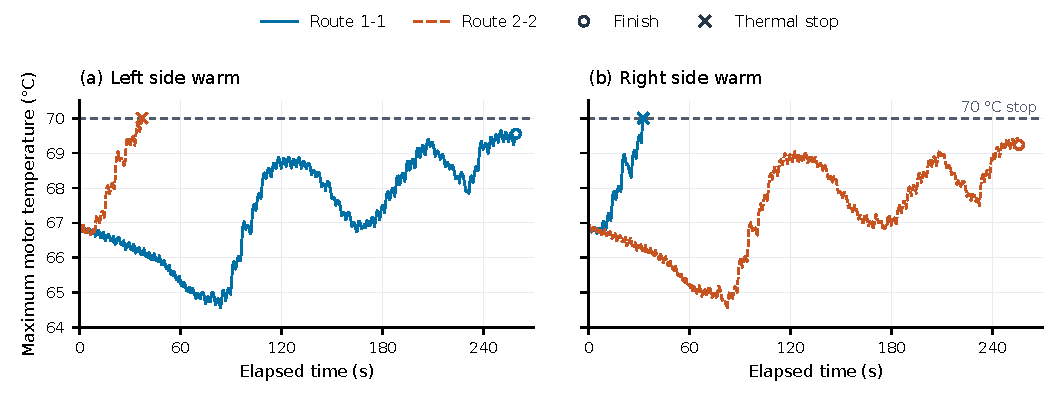
\includegraphics[width=.94\textwidth]{figures/swap_crossover.pdf}
\caption{Thermal crossover on persistent-bank course P3 at heating multiplier 0.46. Each trace shows the hottest motor at each recorded sample. Open circles mark finishes and crosses mark thermal stops. The branch sequence $(1,1)$ finishes left-warm and stops right-warm. The sequence $(2,2)$ has the opposite outcomes.}
\label{fig:crossover}
\end{figure*}

\subsection{Matched Planner Outcomes}

The per-motor planner finished 26 of 72 starts, with two thermal stops and 44 rejections. The aggregate planner finished seven, with five thermal stops and 60 rejections (Table~\ref{tab:planner-results}). Twenty starts finished only with the per-motor planner and one finished only with the aggregate planner. The paired difference of $+26.4$ percentage points had a descriptive 95\% course-resampling interval from $+15.3$ to $+40.3$ points. The experiment met the 10-point practical criterion and recorded three fewer thermal stops.

\begin{table}[!t]
\caption{Planner outcomes across 72 starts per arm}
\label{tab:planner-results}
\centering
\footnotesize
\renewcommand{\arraystretch}{1.13}
\begin{tabular}{@{}lrr@{}}
\hline
Outcome & Mean and maximum & Per motor \\
\hline
Finish & 7 & 26 \\
Thermal stop & 5 & 2 \\
No route admitted & 60 & 44 \\
Other execution failure & 0 & 0 \\
\hline
\end{tabular}
\end{table}

On the 22 starts from pairs requiring different routes, the per-motor planner finished 15 and the aggregate planner finished one. The per-motor planner selected two different routes and finished both starts in six of those pairs. Throughout the entire study it opened up to 10 pairs of start and switchroads. Among the 35 starts with at least one observed finishable route, the per-motor planner finished 26 and rejected seven. It selected a route that stopped thermally on the other two. The aggregate planner rejected 24 of the 35 finishable starts. Selecting routes with full knowledge of the replays could finish 35 starts with an assignment-specific choice, or at most 24 with one route shared per pair.

Fig.~\ref{fig:course-outcomes} shows the distributions across courses. Disjoint finishable sets were most frequent on the persistent-bank courses. In the planner comparison, there were 19 net additional finishes, with seven of them occurring in these courses, and 11 disjoint pairs, with ten of those pairs occurring in these courses.

\begin{figure*}[!t]
\centering
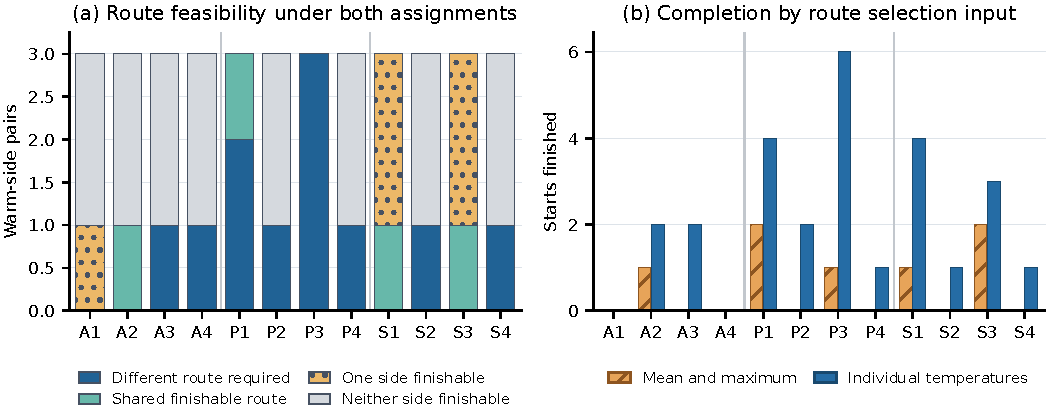
\includegraphics[width=.94\textwidth]{figures/swap_course_outcomes.pdf}
\caption{Outcomes by course. Panel (a) partitions the three thermal-setting pairs on each course by route feasibility. Panel (b) gives the number of finishes by planner over six starts per course. A, P, and S denote alternating banks, persistent banks, and a same-sign stage, respectively.}
\label{fig:course-outcomes}
\end{figure*}

\subsection{Forecast Screening Against Replays}

We applied each planner's admission rule to every route and start, including routes the planner did not select. The maximum possible number of finishable walks is 51, 35 were admitted by the per-motor forecast and 10 by the aggregate forecast (Table~\ref{tab:screening-validation}). Seven of the thermally stopped walks passed the per-motor screen, eight passed the aggregate screen. Each row in Table~\ref{tab:screening-validation} covers 288 route--start combinations. An aggregate score is reused for both starts, and the observed route outcome can differ between the two starts. For the 51 finishes, the per-motor forecasts had a mean absolute peak error of $0.248\,{}^\circ\mathrm{C}$ and a mean absolute arrival error of 3.70 s.

\begin{table}[!t]
\caption{Admission and observed outcome for all 288 warm walks}
\label{tab:screening-validation}
\centering
\footnotesize
\setlength{\tabcolsep}{3pt}
\renewcommand{\arraystretch}{1.15}
\begin{tabular}{@{}lrrrr@{}}
\hline
& \multicolumn{2}{c}{Observed finish} & \multicolumn{2}{c}{Thermal stop} \\
Information & Admit & Reject & Admit & Reject \\
\hline
Mean and maximum & 10 & 41 & 8 & 229 \\
Per-motor temperatures & 35 & 16 & 7 & 230 \\
\hline
\end{tabular}
\end{table}

\subsection{Sensitivity To The Route Screening Cutoff}

We conducted a retrospective check in which we changed the predictive peak-temperature threshold for the admission of a route. Replay outcomes were used with the original forecast. The forecasting and execution target remained unchanged in the speed governor. For every alternative cutoff, we ranked the routes admitted with the original arrivaltime and peak-temperature ranking, and then retrieved the exhaustive replay results.

\begin{table}[!t]
\caption{Retrospective route selection at five forecast cutoffs}
\label{tab:sensitivity}
\centering
\footnotesize
\setlength{\tabcolsep}{3pt}
\renewcommand{\arraystretch}{1.14}
\begin{tabular}{@{}lcccc@{}}
\hline
& \multicolumn{2}{c}{Mean and maximum} & \multicolumn{2}{c}{Per motor} \\
\shortstack{Cutoff\\(\ensuremath{{}^\circ\mathrm{C}})} & Finish & Thermal stop & Finish & Thermal stop \\
\hline
70.00 & 11 & 11 & 33 & 6 \\
69.75 & 7 & 5 & 30 & 3 \\
69.50 & 7 & 5 & 26 & 2 \\
69.25 & 6 & 2 & 11 & 0 \\
69.00 & 5 & 1 & 9 & 0 \\
\hline
\end{tabular}
\end{table}

The per-motor arm finished more starts at all five cutoffs (Table~\ref{tab:sensitivity}). Lowering its cutoff from $69.50$ to $69.25\,{}^\circ\mathrm{C}$ reduced thermal stops from two to zero and reduced completions from 26 to 11. At the more permissive $70.00\,{}^\circ\mathrm{C}$ cutoff it finished 33 starts with six thermal stops. The comparison at $69.50\,{}^\circ\mathrm{C}$ was fixed before the replays. The alternative counts describe the effect of changing the route screen with the walking controller held fixed.

\section{Discussion}

The feasibility result is obtained after performing the same routes with both assignments. For the 11 disjoint pairs and given two indistinguishable summaries, a route rule which must choose one route can end at at most one start. The replay results measure this kind of restriction without being judged on the forecast or cut-off. The aggregate planner's outcome also reflects its equal-weight scoring rule and the chosen forecast cutoff. Its comparison measures the benefit of individual temperatures for these two planners.

Equation~\eqref{eq:thermal-update} gives a mechanism for an effect of the starting assignment. For a fixed torque history, the difference caused by two initial temperatures at motor $i$ decays as $[T_{i,\ell}(0)-T_{i,r}(0)]\exp(-t/\tau)$. The initial contribution combines with the loading of that motor along the route. In the closed-loop replays, changing the temperature also changes the speed command and torque cap, which can change the applied torque history. The two effects are associated with the same physical outcome, and are controlled by the same controller. The motor on the rear right femur first touched the limit on P3 on route $(1,1)$ when it was on the warm side. The left-front femur motor crossed first on route $(2,2)$ with the left side warm. Both stops occurred before the junction. The mixed routes show that completing the approach alone is insufficient.

Disjoint pairs were found in all course families, at all thermal levels. They occurred most often at 0.44 with courses of persistence-banks. Within each setting the model parameters and initial temperatures are set. These combinations are tested to be compared during the experiment. Every forecast was included in the deadline screen and each and every execution was accomplished with a finish or a thermal stop. The results are a description of a thermal feasibility problem on these courses.

\onecolumn
\raggedbottom
\begin{multicols}{2}
The heightfields are synthetic. Thermal parameters are given as inputs to the simulation and initial motor temperatures are provided to the controllers. An assumption of Eq.~\eqref{eq:thermal-update} is that there is no heat transfer between motors. Based on the recorded torques, all 18 temperature histories were recreated by replaying the audit, while checking the completion and termination events. The experiment runs two tests for left--right assignments for two values of temperature. It is the basis of the aggregate comparator of its.

\section{Conclusion}

In the simulated hexapods, which routes they reached when they had the same starting mean and max depended on which side they started warm. On 11 of 36 matched pairs there was a finishable route for each assignment and no shared finishable route. With the same adaptive speed controller during walking, the planner given individual temperatures finished 26 of 72 starts with two thermal stops. The planner given the mean and maximum finished seven with five stops. These results establish the value of preserving the assignment of motor temperatures for route selection under the tested simulated conditions.

\end{multicols}

\appendices

\section{Course Geometry And Finishable Routes}
\label{app:course-data}

The Course Geometry is reported in Table~\ref{tab:geometry}. The length of the projected stage is twice the turn length plus the bank length and an allowance of 1m for landing. Two types of offsets are lateral centerline displacements. Bank shifts move the bank envelope up or down each of the branches. The angle - symbols indicate the direction of the height gradient of the lateral coordinate.

\begin{appendixdisplay}{table}
\caption{Geometry of the twelve hot-motor swap courses}
\label{tab:geometry}
\centering
\footnotesize
\setlength{\tabcolsep}{4pt}
\renewcommand{\arraystretch}{1.00}
\begin{tabular*}{\linewidth}{@{\extracolsep{\fill}}lrrrrrrrrrr@{}}
\hline
& & \multicolumn{3}{c}{Longitudinal geometry} & \multicolumn{2}{c}{Offsets (m)} & \multicolumn{2}{c}{Bank angles (deg)} & \multicolumn{2}{c}{Bank shifts (m)} \\
\cline{3-5}\cline{6-7}\cline{8-9}\cline{10-11}
Course & Stage & Turn (m) & Bank (m) & Deadline (s) & Branch 1 & Branch 2 & Branch 1 & Branch 2 & Branch 1 & Branch 2 \\
\hline
A1 & 1 & 6.77 & 5.14 & 358 & $-2.15$ & $2.23$ & $-8.38$ & $8.17$ & $0.01$ & $-0.17$ \\
 & 2 & 6.74 & 4.51 &  & $-2.12$ & $2.12$ & $7.86$ & $-7.90$ & $0.44$ & $-0.30$ \\
A2 & 1 & 7.05 & 4.76 & 358 & $-2.23$ & $2.14$ & $8.18$ & $-8.92$ & $-0.45$ & $-0.30$ \\
 & 2 & 6.80 & 4.17 &  & $-2.19$ & $2.27$ & $-8.54$ & $8.31$ & $0.07$ & $0.33$ \\
A3 & 1 & 6.71 & 4.37 & 358 & $-2.33$ & $2.22$ & $-7.56$ & $7.31$ & $0.30$ & $-0.43$ \\
 & 2 & 7.08 & 4.70 &  & $-2.25$ & $2.26$ & $7.90$ & $-8.63$ & $0.08$ & $0.20$ \\
A4 & 1 & 6.53 & 4.53 & 352 & $-2.34$ & $2.31$ & $7.41$ & $-7.67$ & $-0.22$ & $0.26$ \\
 & 2 & 6.80 & 4.84 &  & $-2.22$ & $2.25$ & $-7.36$ & $7.94$ & $0.38$ & $0.16$ \\
\hline
P1 & 1 & 6.97 & 4.84 & 353 & $-2.26$ & $2.23$ & $-9.54$ & $8.87$ & $0.04$ & $0.40$ \\
 & 2 & 6.45 & 4.46 &  & $-2.33$ & $2.13$ & $-8.16$ & $7.55$ & $0.10$ & $0.13$ \\
P2 & 1 & 6.92 & 5.00 & 358 & $-2.28$ & $2.34$ & $8.50$ & $-7.86$ & $-0.07$ & $0.42$ \\
 & 2 & 6.80 & 4.20 &  & $-2.24$ & $2.28$ & $8.64$ & $-7.61$ & $0.34$ & $-0.09$ \\
P3 & 1 & 6.55 & 4.57 & 355 & $-2.20$ & $2.23$ & $-8.15$ & $8.49$ & $0.33$ & $-0.08$ \\
 & 2 & 6.91 & 4.89 &  & $-2.36$ & $2.14$ & $-8.59$ & $8.47$ & $-0.18$ & $0.27$ \\
P4 & 1 & 6.51 & 4.31 & 355 & $-2.33$ & $2.24$ & $9.10$ & $-7.39$ & $-0.26$ & $-0.19$ \\
 & 2 & 6.95 & 5.11 &  & $-2.18$ & $2.25$ & $9.03$ & $-7.79$ & $0.28$ & $-0.33$ \\
\hline
S1 & 1 & 6.86 & 4.80 & 353 & $-2.29$ & $2.30$ & $-8.20$ & $-9.11$ & $-0.28$ & $-0.21$ \\
 & 2 & 6.60 & 4.39 &  & $-2.16$ & $2.26$ & $-8.36$ & $8.80$ & $-0.31$ & $0.18$ \\
S2 & 1 & 7.38 & 5.19 & 364 & $-2.29$ & $2.23$ & $7.84$ & $8.12$ & $0.00$ & $0.19$ \\
 & 2 & 6.49 & 4.41 &  & $-2.23$ & $2.15$ & $7.90$ & $-8.36$ & $0.32$ & $0.24$ \\
S3 & 1 & 6.57 & 4.31 & 356 & $-2.21$ & $2.35$ & $-9.01$ & $8.71$ & $0.11$ & $-0.30$ \\
 & 2 & 7.17 & 4.63 &  & $-2.12$ & $2.19$ & $-8.14$ & $-7.28$ & $0.31$ & $0.02$ \\
S4 & 1 & 6.73 & 4.57 & 366 & $-2.21$ & $2.36$ & $7.83$ & $-9.04$ & $-0.09$ & $0.05$ \\
 & 2 & 7.18 & 5.17 &  & $-2.18$ & $2.18$ & $7.36$ & $8.04$ & $0.36$ & $-0.22$ \\
\hline
\end{tabular*}
\end{appendixdisplay}

\begin{appendixdisplay}{table}
The list of routes (including those that neither planner admitted) ending among the 288 warm replays is given in table~\ref{tab:finishable-routes}.\par
\caption{Finishable routes for both assignments at every setting}
\label{tab:finishable-routes}
\centering
\footnotesize
\setlength{\tabcolsep}{4pt}
\renewcommand{\arraystretch}{1.00}
\begin{tabular*}{\linewidth}{@{\extracolsep{\fill}}lcccccc@{}}
\hline
& \multicolumn{2}{c}{Heating 0.44} & \multicolumn{2}{c}{Heating 0.45} & \multicolumn{2}{c}{Heating 0.46} \\
\cline{2-3}\cline{4-5}\cline{6-7}
Course & Left warm & Right warm & Left warm & Right warm & Left warm & Right warm \\
\hline
A1 & 4 & $\varnothing$ & $\varnothing$ & $\varnothing$ & $\varnothing$ & $\varnothing$ \\
A2 & 1, 3, 4 & 2, 4 & $\varnothing$ & $\varnothing$ & $\varnothing$ & $\varnothing$ \\
A3 & 4 & 1 & $\varnothing$ & $\varnothing$ & $\varnothing$ & $\varnothing$ \\
A4 & 3, 4 & 1, 2 & $\varnothing$ & $\varnothing$ & $\varnothing$ & $\varnothing$ \\
P1 & 1, 3, 4 & 4 & 1 & 4 & 1 & 4 \\
P2 & 4 & 1 & $\varnothing$ & $\varnothing$ & $\varnothing$ & $\varnothing$ \\
P3 & 1, 3 & 2, 4 & 1 & 4 & 1 & 4 \\
P4 & 4 & 1, 2 & $\varnothing$ & $\varnothing$ & $\varnothing$ & $\varnothing$ \\
S1 & 1, 3, 4 & 2, 4 & 1 & $\varnothing$ & 1 & $\varnothing$ \\
S2 & 4 & 1, 2 & $\varnothing$ & $\varnothing$ & $\varnothing$ & $\varnothing$ \\
S3 & 1 & 1, 2 & 1 & $\varnothing$ & 1 & $\varnothing$ \\
S4 & 3 & 1, 2 & $\varnothing$ & $\varnothing$ & $\varnothing$ & $\varnothing$ \\
\hline
\end{tabular*}
\par\smallskip
\parbox{\linewidth}{\raggedright Routes 1 through 4 denote $(1,1)$, $(1,2)$, $(2,1)$, and $(2,2)$, respectively. $\varnothing$ indicates that every route reached the thermal limit.}
\end{appendixdisplay}

\begin{multicols}{2}
\section{Matched Junction-Pause Experiment}
\label{app:pause}

A separate experiment compared route selection with and without a planned 12 s pause on 12 other two-stage courses. Both arms used the adapted speed governor, the $69.50\,{}^\circ\mathrm{C}$ forecast cutoff, the deadline, and the same route ranking. On each route, both rates of pausing were assessed by the optional arm and a zero pause size was preferred on the same route. The individual starting temperatures were used for both arms. The course lengths were 37.44--40.29 m. Deadlines used the same rule for projected-length as the main experiment. 72 starts were provided by the application of the 12 courses on both sides at the three thermal levels. With this earlier pause protocol, each arm had the same number of online seconds of budget: two.

When at the flat junction with a ``paused'' replay, the controller sent a signal to step forward at zero speed. The break was counted towards deadline. The forecast position was kept at the same forward cross position and the motor load was fitted for 24 prediction steps and the governor clock was advanced. Immediately following the pause button it resumed the evolved temperatures and speed state. Forecast peak included approach, pause and departure.

For each of eight recorded 12 s pause windows on one development approach, four per approach speed, we used the simulated entry and exit temperatures, $T_{i,\mathrm{in}}$ and $T_{i,\mathrm{out}}$, to estimate the constant squared torque $q_{i,\mathrm{hold}}^2$ for a pause of duration $d$.

\begin{equation}
q_{i,\mathrm{hold}}^2 =
\frac{q_{\mathrm{ref}}^2}{R}
\left[T_{i,\mathrm{in}}-T_{\mathrm{amb}}+
\frac{T_{i,\mathrm{out}}-T_{i,\mathrm{in}}}{1-\exp(-d/\tau)}\right].
\end{equation}

We averaged inferred squared torques within each approach speed and then weighted the two speeds equally. The paused forecasts used those fitted loads (Table~\ref{tab:hold-loads}). Equation~\eqref{eq:thermal-update} predicts cooling for a motor when its junction-entry temperature exceeds the equilibrium implied by the hold load. At pause exit, the forecast resumes progress with the evolved temperature vector and current speed state. It evaluates the cutoff over the entire prediction, including the initial stand and the pause.

\begin{appendixdisplay}{table}
\caption{Fitted squared torque during a 12 s hold in $(\mathrm{N}{\cdot}\mathrm{m})^2$}
\label{tab:hold-loads}
\centering
\footnotesize
\renewcommand{\arraystretch}{1.12}
\begin{tabular*}{\linewidth}{@{\extracolsep{\fill}}lrrr@{}}
\hline
Leg & Coxa & Femur & Tibia \\
\hline
Left front & 5.943 & 2904.157 & 28.293 \\
Left middle & 3.320 & 3758.819 & 34.013 \\
Left rear & 1.669 & 2809.037 & 27.238 \\
Right front & 2.627 & 3030.600 & 29.827 \\
Right middle & 1.695 & 3578.708 & 34.374 \\
Right rear & 2.913 & 2911.345 & 29.891 \\
\hline
\end{tabular*}
\end{appendixdisplay}

The optional-pause arm finished 29 starts with four thermal stops and 39 rejections. The no-pause arm finished 25 with two thermal stops and 45 rejections. All 25 starts that finished under the no-pause arm also finished under the optional arm. The four additional finishes gave a gain of 5.6 percentage points. Gain was less than the target 10 points and the number of thermal-stops was two higher.

27 hits were put through the no-pause arm. The optional arm kept their slate and opted to pick up six passed starts. There were 27 equal games with one each replay. All pauses were 12 s long. Each of the six selected routes was rerun without any stops, with the same starting temperatures and controller. The total quantity of 39 different physics replays and the six diagnostics was obtained. The paired traces were in accordance with the sample just preceding the pause. These diagnostics are in addition to the arm's counts, and will not be paused by the arm.

\end{multicols}

\begin{appendixdisplay}{table}
\caption{Fixed-route diagnostic for the six selected pauses}
\label{tab:matched-same-route}
\centering
\setlength{\tabcolsep}{4pt}
\footnotesize
\renewcommand{\arraystretch}{1.12}
\begin{tabular*}{\linewidth}{@{\extracolsep{\fill}}llrrrrll@{}}
\hline
& & \multicolumn{2}{c}{Forecast peak (\ensuremath{{}^{\circ}\mathrm{C}})}
  & \multicolumn{2}{c}{Observed peak (\ensuremath{{}^{\circ}\mathrm{C}})}
  & \multicolumn{2}{c}{Physics outcome} \\
\cline{3-4}\cline{5-6}\cline{7-8}
Course & Start & 0 s & 12 s & 0 s & 12 s & 0 s & 12 s \\
\hline
Alternating balanced & 0.44 left & 69.553 & 69.096 & 70.014 & 69.304 & Thermal stop & Finish \\
Alternating long exit & 0.44 right & 70.377 & 69.486 & 70.001 & 69.663 & Thermal stop & Finish \\
Alternating long exit & 0.45 left & 70.914 & 69.483 & 70.009 & 70.000 & Thermal stop & Thermal stop \\
Shared entry & 0.44 right & 69.552 & 69.469 & 69.860 & 69.830 & Finish & Finish \\
Shared entry & 0.45 left & 71.376 & 69.378 & 70.009 & 70.001 & Thermal stop & Thermal stop \\
Shared long exit & 0.44 right & 70.136 & 69.492 & 70.011 & 69.962 & Thermal stop & Finish \\
\hline
\end{tabular*}

\par\smallskip
\parbox{\linewidth}{\raggedright Start is warming relative to heating and the side that is initially warmer. None of the zero-pause forecasts in this table met the 69.50 \ensuremath{{}^{\circ}\mathrm{C}} gate. They have been replayed as diagnostics and aren't included in control-arm attempts. Thermal stops are observed peaks through the first sample on or higher than 70 \ensuremath{{}^{\circ}\mathrm{C}}.}
\end{appendixdisplay}

\begin{appendixdisplay}{figure}
\centering
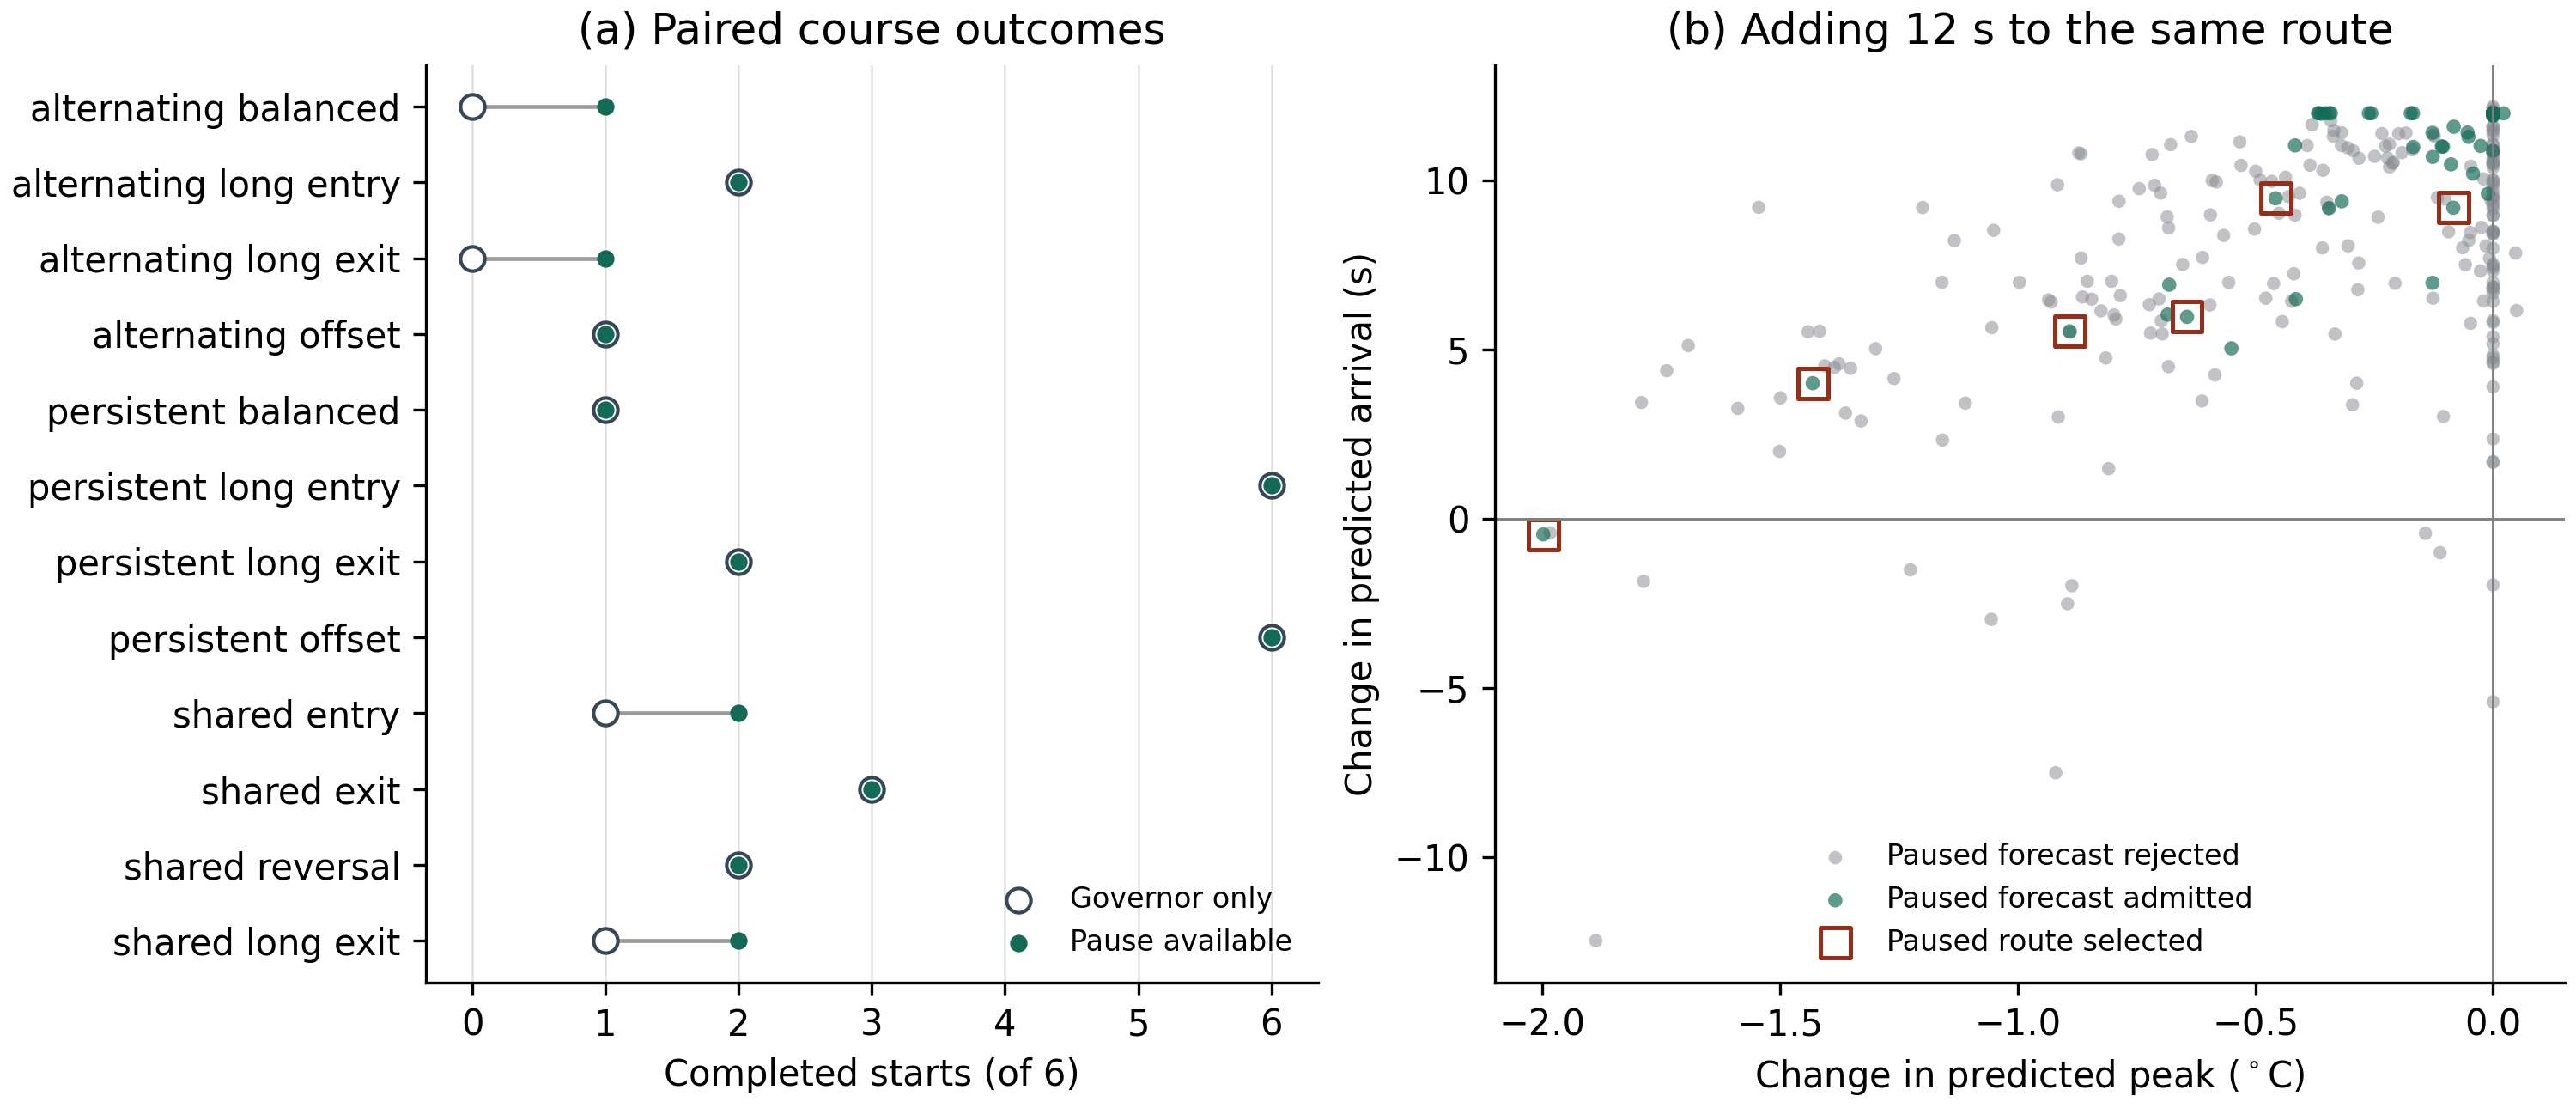
\includegraphics[width=.98\textwidth]{figures/matched_pause_outcomes.png}
\caption{Supporting junction-pause experiment on 12 courses. Panel (a) gives the number of completed starts per course. Panel (b) shows the forecast change from adding a 12 s pause to the same route for each of the 288 route-and-start pairs. Negative peak changes indicate a lower predicted peak motor temperature. Six paused plans were selected.}
\label{fig:matched}
\end{appendixdisplay}

\begin{multicols}{2}
\raggedcolumns

Three selected routes changed from a thermal stop to a finish in their same-route diagnostic, one finished at both durations, and two stopped thermally at both durations (Table~\ref{tab:matched-same-route}). The motor that was hottest at pause entry cooled by $1.01$--$1.44\,{}^\circ\mathrm{C}$ over the pause. In the two stopped paused walks, the motor later reached the thermal threshold after walking resumed. Forecast peaks for those two paused walks were about $0.52$ and $0.62\,{}^\circ\mathrm{C}$ below the recorded peaks at the thermal stop. One additional finish, on the shared-entry course, came from admitting a paused route whose zero-pause version also finished in its diagnostic. Its zero-pause forecast peak was $69.552\,{}^\circ\mathrm{C}$, just above the forecast cutoff.

The time-only fallback in the earlier comparison also allowed a diagnosis on 48 fixed schedules. Applying the full paused forecast at $69.50\,{}^\circ\mathrm{C}$ rejected 38 thermal stops and nine finishable schedules, while admitting one finishable schedule. At $70.00\,{}^\circ\mathrm{C}$, the same forecasts admitted ten finishes and one thermal stop. The diagnostic kept the candidate schedules fixed. It measures the screening trade-off on these schedules.

\columnbreak
\section{Earlier Routing And Pause Comparisons}
\label{app:earlier-benchmark}

Previous development test programs involved one split on six courses, to which each had a different thermal setting. Only one finishable branch was changed in 15 out of 54 pairs of branches that were matched. In a subsequent network experiment, the planner chose routes as well as discrete speed schedules with both employing a reactive slowdown policy during the walk. With an individual motor temperature, the planner completed 32-36 starts. A planner who made average thermal forecasts over the two potential assignments finished 31. The total of all whole circuits are examined in the current experiment for both assignments on an individual course set with the same adjusted speed governor for planning in both planners.

The pause benchmark mentioned above is summarized in Table~\ref{tab:earlier-planners}. The same reactive execution controller was employed in conjunction to the first three planners. Of the 38 time-only fallback walks that stopped, ten reached the junction. The adapted speed rule reused the same 72 starts and ranked candidates by predicted arrival. Its route ranking and execution controller differed from those used by the first three planners.

\begin{appendixdisplay}{table}
\caption{Earlier planner comparison over 72 starts per method}
\label{tab:earlier-planners}
\centering
\footnotesize
\renewcommand{\arraystretch}{1.13}
\begin{tabular*}{\linewidth}{@{\extracolsep{\fill}}lrr@{}}
\hline
Planner & Finish & Thermal stop \\
\hline
Fixed reactive & 18 & 0 \\
Time-only pause fallback & 28 & 38 \\
Thermally screened pause fallback & 20 & 0 \\
Adapted thermal speed rule & 30 & 3 \\
\hline
\end{tabular*}
\end{appendixdisplay}

\end{multicols}

\twocolumn
\raggedbottom
\begin{thebibliography}{00}
\interlinepenalty=10000
\bibitem{trujillo2009}
S. Trujillo and M. Cutkosky, \textquotedblleft{}Thermally constrained motor operation for a climbing robot,\textquotedblright{} in \emph{Proc. IEEE Int. Conf. Robot. Autom.}, May 2009, pp. 2362--2367, doi: \href{https://doi.org/10.1109/ROBOT.2009.5152870}{\nolinkurl{10.1109/ROBOT.2009.5152870}}.

\bibitem{mellor1991}
P. H. Mellor, D. Roberts, and D. R. Turner, \textquotedblleft{}Lumped parameter thermal model for electrical machines of TEFC design,\textquotedblright{} \emph{IEE Proc. B, Electr. Power Appl.}, vol. 138, no. 5, pp. 205--218, 1991, doi: \href{https://doi.org/10.1049/ip-b.1991.0025}{\nolinkurl{10.1049/ip-b.1991.0025}}.

\bibitem{de2011}
A. De, G. Lynch, A. Johnson, and D. Koditschek, \textquotedblleft{}Motor sizing for legged robots using dynamic task specification,\textquotedblright{} in \emph{Proc. IEEE Int. Conf. Technol. Practical Robot Appl.}, Apr. 2011, pp. 64--69, doi: \href{https://doi.org/10.1109/TEPRA.2011.5753483}{\nolinkurl{10.1109/TEPRA.2011.5753483}}.

\bibitem{lin2025}
W. Lin, L. Qian, X. Luo, and C. Liang, \textquotedblleft{}Temperature distribution prediction of the quadruped robot based on the lumped-parameter thermal networks,\textquotedblright{} \emph{Robot}, vol. 47, no. 2, pp. 188--199, 2025, doi: \href{https://robot.sia.cn/en/article/doi/10.13973/j.cnki.robot.240208}{\nolinkurl{10.13973/j.cnki.robot.240208}}.

\bibitem{tan2018heat}
W. X. Tan, M. Brandão, K. Hashimoto, and A. Takanishi, \textquotedblleft{}Trajectory optimization for high-power robots with motor temperature constraints,\textquotedblright{} in \emph{Proc. Towards Auton. Robot. Syst. (TAROS)}, 2018, pp. 3--14, doi: \href{https://doi.org/10.1007/978-3-319-96728-8_1}{\nolinkurl{10.1007/978-3-319-96728-8_1}}.

\bibitem{kawaharazuka2020}
K. Kawaharazuka \emph{et al.}, \textquotedblleft{}Estimation and control of motor core temperature with online learning of thermal model parameters: Application to musculoskeletal humanoids,\textquotedblright{} \emph{IEEE Robot. Autom. Lett.}, vol. 5, no. 3, pp. 4273--4280, 2020, doi: \href{https://doi.org/10.1109/LRA.2020.2990889}{\nolinkurl{10.1109/LRA.2020.2990889}}.

\bibitem{debenedittis2026}
D. De Benedittis, F. Angelini, R. Incerpi, L. Pallottino, and M. Garabini, \textquotedblleft{}Keep it cool: Optimal control of robotic systems under temperature constraints,\textquotedblright{} \emph{IEEE Trans. Control Syst. Technol.}, vol. 34, no. 6, pp. 3128--3139, Nov. 2026, doi: \href{https://doi.org/10.1109/TCST.2026.3721130}{\nolinkurl{10.1109/TCST.2026.3721130}}.

\bibitem{wan2026}
Y. Wan \emph{et al.}, \textquotedblleft{}Learning to balance motor thermal safety and quadrupedal locomotion performance with residual policy,\textquotedblright{} arXiv preprint \href{https://arxiv.org/abs/2605.27046v3}{arXiv:2605.27046v3}, 2026.

\bibitem{segas2026}
R. Ségas, B. Opra, L. Ghafari, and T. Stewart, \textquotedblleft{}From temperature-limited to battery-limited legged locomotion,\textquotedblright{} arXiv preprint \href{https://arxiv.org/abs/2611.22231}{arXiv:2611.22231}, 2026.

\bibitem{faigl2019}
J. Faigl and P. Čížek, \textquotedblleft{}Adaptive locomotion control of hexapod walking robot for traversing rough terrains with position feedback only,\textquotedblright{} \emph{Robot. Auton. Syst.}, vol. 116, pp. 136--147, 2019, doi: \href{https://doi.org/10.1016/j.robot.2019.03.008}{\nolinkurl{10.1016/j.robot.2019.03.008}}.

\bibitem{brodoline2024}
I. Brodoline, E. Sauvageot, S. Viollet, and J. R. Serres, \textquotedblleft{}Shaping the energy curves of a servomotor-based hexapod robot,\textquotedblright{} \emph{Sci. Rep.}, vol. 14, no. 1, Art. no. 11675, 2024, doi: \href{https://doi.org/10.1038/s41598-024-62184-y}{\nolinkurl{10.1038/s41598-024-62184-y}}.

\bibitem{jorgensen2019}
S. J. Jorgensen, J. Holley, F. Mathis, J. S. Mehling, and L. Sentis, \textquotedblleft{}Thermal recovery of multi-limbed robots with electric actuators,\textquotedblright{} \emph{IEEE Robot. Autom. Lett.}, vol. 4, no. 2, pp. 1077--1084, 2019, doi: \href{https://doi.org/10.1109/LRA.2019.2894068}{\nolinkurl{10.1109/LRA.2019.2894068}}.

\bibitem{urata2017}
J. Urata and Y. Ito, \textquotedblleft{}Determining a trajectory for a walking robot to prevent motor overheating,\textquotedblright{} U.S. Patent 9\,821\,461 B1, Nov. 21, 2017. \href{https://patents.google.com/patent/US9821461B1/en}{US9821461B1}.

\bibitem{zhao2021}
Y. Zhao, F. Gao, Q. Sun, and Y. Yin, \textquotedblleft{}Terrain classification and adaptive locomotion for a hexapod robot Qingzhui,\textquotedblright{} \emph{Front. Mech. Eng.}, vol. 16, no. 2, pp. 271--284, 2021, doi: \href{https://doi.org/10.1007/s11465-020-0623-1}{\nolinkurl{10.1007/s11465-020-0623-1}}.

\bibitem{ding2024}
L. Ding \emph{et al.}, \textquotedblleft{}Motion planning and contact force distribution for heavy-duty hexapod robots walking on unknown rugged terrains,\textquotedblright{} \emph{J. Field Robot.}, vol. 41, no. 6, pp. 1680--1701, 2024, doi: \href{https://doi.org/10.1002/rob.22338}{\nolinkurl{10.1002/rob.22338}}.

\bibitem{gehring2015}
C. Gehring \emph{et al.}, \textquotedblleft{}Dynamic trotting on slopes for quadrupedal robots,\textquotedblright{} in \emph{Proc. IEEE/RSJ Int. Conf. Intell. Robots Syst.}, Sep. 2015, pp. 5129--5135, doi: \href{https://doi.org/10.1109/IROS.2015.7354099}{\nolinkurl{10.1109/IROS.2015.7354099}}.

\bibitem{focchi2017}
M. Focchi, A. del Prete, I. Havoutis, R. Featherstone, D. G. Caldwell, and C. Semini, \textquotedblleft{}High-slope terrain locomotion for torque-controlled quadruped robots,\textquotedblright{} \emph{Auton. Robots}, vol. 41, no. 1, pp. 259--272, 2017, doi: \href{https://doi.org/10.1007/s10514-016-9573-1}{\nolinkurl{10.1007/s10514-016-9573-1}}.

% Start the second reference column between complete entries.
\newpage
\bibitem{righetti2013}
L. Righetti, J. Buchli, M. Mistry, M. Kalakrishnan, and S. Schaal, \textquotedblleft{}Optimal distribution of contact forces with inverse-dynamics control,\textquotedblright{} \emph{Int. J. Robot. Res.}, vol. 32, no. 3, pp. 280--298, 2013, doi: \href{https://doi.org/10.1177/0278364912469821}{\nolinkurl{10.1177/0278364912469821}}.

\bibitem{luneckas2019}
M. Luneckas, T. Luneckas, D. Udris, D. Plonis, R. Maskeliunas, and R. Damasevicius, \textquotedblleft{}Energy-efficient walking over irregular terrain: a case of hexapod robot,\textquotedblright{} \emph{Metrol. Meas. Syst.}, vol. 26, no. 4, pp. 645--660, 2019, doi: \href{https://doi.org/10.24425/mms.2019.130562}{\nolinkurl{10.24425/mms.2019.130562}}.

\bibitem{luneckas2021}
M. Luneckas \emph{et al.}, \textquotedblleft{}Hexapod robot gait switching for energy consumption and cost of transport management using heuristic algorithms,\textquotedblright{} \emph{Appl. Sci.}, vol. 11, no. 3, Art. no. 1339, 2021, doi: \href{https://doi.org/10.3390/app11031339}{\nolinkurl{10.3390/app11031339}}.

\bibitem{seok2015}
S. Seok \emph{et al.}, \textquotedblleft{}Design principles for energy-efficient legged locomotion and implementation on the MIT Cheetah robot,\textquotedblright{} \emph{IEEE/ASME Trans. Mechatronics}, vol. 20, no. 3, pp. 1117--1129, 2015, doi: \href{https://doi.org/10.1109/TMECH.2014.2339013}{\nolinkurl{10.1109/TMECH.2014.2339013}}.

\bibitem{schperberg2025}
A. Schperberg, M. Menner, and S. D. Di Cairano, \textquotedblleft{}Energy-efficient motion planner for legged robots,\textquotedblright{} in \emph{Proc. IEEE/RSJ Int. Conf. Intell. Robots Syst.}, Oct. 2025, pp. 18888--18895, doi: \href{https://doi.org/10.1109/IROS60139.2025.11246509}{\nolinkurl{10.1109/IROS60139.2025.11246509}}.

\bibitem{hauser2008}
K. Hauser, T. Bretl, J.-C. Latombe, K. Harada, and B. Wilcox, \textquotedblleft{}Motion planning for legged robots on varied terrain,\textquotedblright{} \emph{Int. J. Robot. Res.}, vol. 27, no. 11--12, pp. 1325--1349, 2008, doi: \href{https://doi.org/10.1177/0278364908098447}{\nolinkurl{10.1177/0278364908098447}}.

\bibitem{valouch2021}
D. Valouch and J. Faigl, \textquotedblleft{}Gait-free planning for hexapod walking robot,\textquotedblright{} in \emph{Proc. Eur. Conf. Mobile Robots}, Aug. 2021, pp. 1--8, doi: \href{https://doi.org/10.1109/ECMR50962.2021.9568834}{\nolinkurl{10.1109/ECMR50962.2021.9568834}}.

\bibitem{jenelten2020}
F. Jenelten, T. Miki, A. E. Vijayan, M. Bjelonic, and M. Hutter, \textquotedblleft{}Perceptive locomotion in rough terrain -- Online foothold optimization,\textquotedblright{} \emph{IEEE Robot. Autom. Lett.}, vol. 5, no. 4, pp. 5370--5376, 2020, doi: \href{https://doi.org/10.1109/LRA.2020.3007427}{\nolinkurl{10.1109/LRA.2020.3007427}}.

\bibitem{mastalli2020}
C. Mastalli, I. Havoutis, M. Focchi, D. G. Caldwell, and C. Semini, \textquotedblleft{}Motion planning for quadrupedal locomotion: Coupled planning, terrain mapping, and whole-body control,\textquotedblright{} \emph{IEEE Trans. Robot.}, vol. 36, no. 6, pp. 1635--1648, 2020, doi: \href{https://doi.org/10.1109/TRO.2020.3003464}{\nolinkurl{10.1109/TRO.2020.3003464}}.

\bibitem{brandao2016}
M. Brandão, K. Hashimoto, J. Santos-Victor, and A. Takanishi, \textquotedblleft{}Footstep planning for slippery and slanted terrain using human-inspired models,\textquotedblright{} \emph{IEEE Trans. Robot.}, vol. 32, no. 4, pp. 868--879, 2016, doi: \href{https://doi.org/10.1109/TRO.2016.2581219}{\nolinkurl{10.1109/TRO.2016.2581219}}.

\bibitem{pragr2022}
M. Prágr, J. Bayer, and J. Faigl, \textquotedblleft{}Autonomous robotic exploration with simultaneous environment and traversability models learning,\textquotedblright{} \emph{Front. Robot. AI}, vol. 9, Art. no. 910113, 2022, doi: \href{https://doi.org/10.3389/frobt.2022.910113}{\nolinkurl{10.3389/frobt.2022.910113}}.

\bibitem{fu2022}
Z. Fu, A. Kumar, A. Agarwal, H. Qi, J. Malik, and D. Pathak, \textquotedblleft{}Coupling vision and proprioception for navigation of legged robots,\textquotedblright{} in \emph{Proc. IEEE/CVF Conf. Comput. Vis. Pattern Recognit.}, Jun. 2022, pp. 17252--17262, doi: \href{https://doi.org/10.1109/CVPR52688.2022.01676}{\nolinkurl{10.1109/CVPR52688.2022.01676}}.

\bibitem{yang2021}
B. Yang, L. Wellhausen, T. Miki, M. Liu, and M. Hutter, \textquotedblleft{}Real-time optimal navigation planning using learned motion costs,\textquotedblright{} in \emph{Proc. IEEE Int. Conf. Robot. Autom.}, May 2021, pp. 9283--9289, doi: \href{https://doi.org/10.1109/ICRA48506.2021.9561861}{\nolinkurl{10.1109/ICRA48506.2021.9561861}}.

\bibitem{david2022}
J. David, T. Bridgwater, A. West, B. Lennox, and M. Giuliani, \textquotedblleft{}Internal state-based risk assessment for robots in hazardous environment,\textquotedblright{} in \emph{Proc. Towards Auton. Robot. Syst. (TAROS)}, vol. 13546, Cham, Switzerland, Springer, 2022, pp. 137--152, doi: \href{https://doi.org/10.1007/978-3-031-15908-4_12}{\nolinkurl{10.1007/978-3-031-15908-4_12}}.

\bibitem{todorov2012}
E. Todorov, T. Erez, and Y. Tassa, \textquotedblleft{}MuJoCo: A physics engine for model-based control,\textquotedblright{} in \emph{Proc. IEEE/RSJ Int. Conf. Intell. Robots Syst.}, Oct. 2012, pp. 5026--5033, doi: \href{https://doi.org/10.1109/IROS.2012.6386109}{\nolinkurl{10.1109/IROS.2012.6386109}}.

\bibitem{mcmordie2003}
D. McMordie, C. Prahacs, and M. Buehler, \textquotedblleft{}Towards a dynamic actuator model for a hexapod robot,\textquotedblright{} in \emph{Proc. IEEE Int. Conf. Robot. Autom.}, vol. 1, 2003, pp. 1386--1390, doi: \href{https://doi.org/10.1109/ROBOT.2003.1241785}{\nolinkurl{10.1109/ROBOT.2003.1241785}}.

\bibitem{hwangbo2019}
J. Hwangbo \emph{et al.}, \textquotedblleft{}Learning agile and dynamic motor skills for legged robots,\textquotedblright{} \emph{Sci. Robot.}, vol. 4, no. 26, Art. no. eaau5872, 2019, doi: \href{https://doi.org/10.1126/scirobotics.aau5872}{\nolinkurl{10.1126/scirobotics.aau5872}}.
\end{thebibliography}

\clearpage
\pdfbookmark[1]{Author Biographies}{author-biographies}
\begingroup
\hypersetup{bookmarksdepth=1}
\makeatletter
\renewcommand{\@IEEEBIOskipN}{.5\baselineskip}
\makeatother
% Author biographies and portraits from the supplied Word document, in byline order.

\begin{biography}[{
\includegraphics[width=1in,height=1.25in,keepaspectratio,clip]{figures/authors/foo-jin-wayne.jpg}}]{Foo Jin Wayne}
is pursuing a diploma in computer science.

He is with the Research Centre for Human-Machine Collaboration (HUMAC), Faculty of Engineering and Technology, Sunway University, Bandar Sunway, Malaysia. His research focuses on simulated hexapod locomotion and route planning that accounts for individual motor temperatures. He is investigating whether training with deformable soil models improves hexapod walking performance on unfamiliar terrain.
\end{biography}

\begin{biography}[{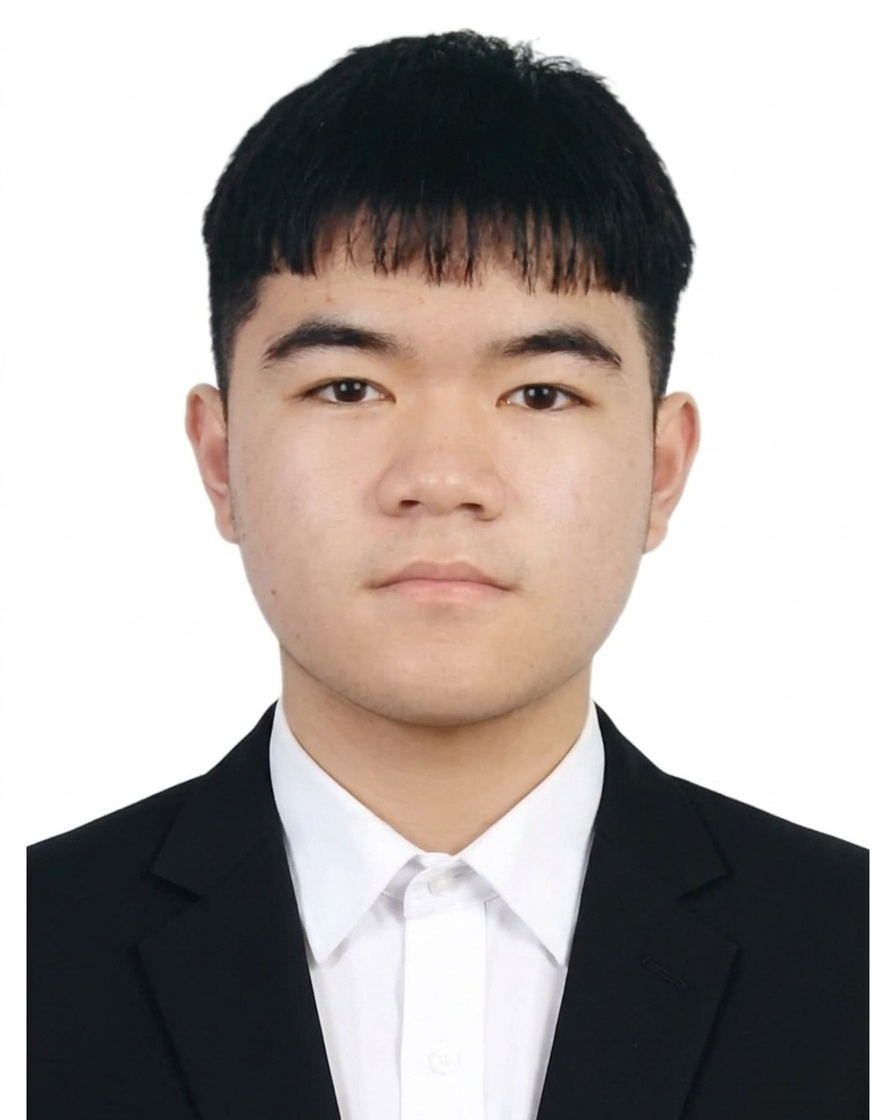
\includegraphics[width=1in,height=1.25in,keepaspectratio,clip]{figures/authors/juo-wei-lai.jpg}}]{Juo Wei Lai}
is affiliated with the research centre for human machine collaboration (HUMAC), Faculty of engineering and Technology, Bandar Sunway, Malaysia [Diploma in Information Technology, Jan 2025]. His research focuses more towards mobile robot navigation, coverage path, and simulation for hexapod inspection applications. Through the project of MINIS, he explores more on mission planning for browser-based, waypoint execution, and synthetic inspection mapping, with an emphasis on system behaviour and reproducible evaluation of simulation results.
\end{biography}

\begin{biography}[{
\includegraphics[width=1in,height=1.25in,keepaspectratio,clip]{figures/authors/latifah-mohammed-abdulrahman.jpg}}]{Latifah Mohammed Abdulrahman}
has undertaken diploma studies in computer science.

She is with the Research Centre for Human-Machine Collaboration (HUMAC), Faculty of Engineering and Technology, Sunway University, Bandar Sunway, Malaysia. She studies dynamic jumping on a simulated 18-joint hexapod using central pattern generators, geometric foot steering, landing feedback, and bounded corrections learned through proximal policy optimization. Her work compares residual joint control, oscillator parameter modulation, and direct position control for continuous multihop jumping, directional control, and landing recovery across four jumping stages.
\end{biography}

\begin{biography}[{
\includegraphics[width=1in,height=1.25in,keepaspectratio,clip]{figures/authors/gulhajar-melebayeva.jpg}}]{Gulhajar Melebayeva}
has undertaken diploma studies in information technology.

She is an intern with the Research Centre for Human-Machine Collaboration (HUMAC), Faculty of Engineering and Technology, Sunway University, Bandar Sunway, Malaysia. Her research combines bioinspired central pattern generators with deep reinforcement learning for multilegged robots. She studies bounded residual reinforcement learning, continuous multistage jumping, and contact recovery, and assesses controller robustness and numerical sensitivity in rigid-body simulations of 18-degree-of-freedom hexapods.
\end{biography}

\begin{biography}[{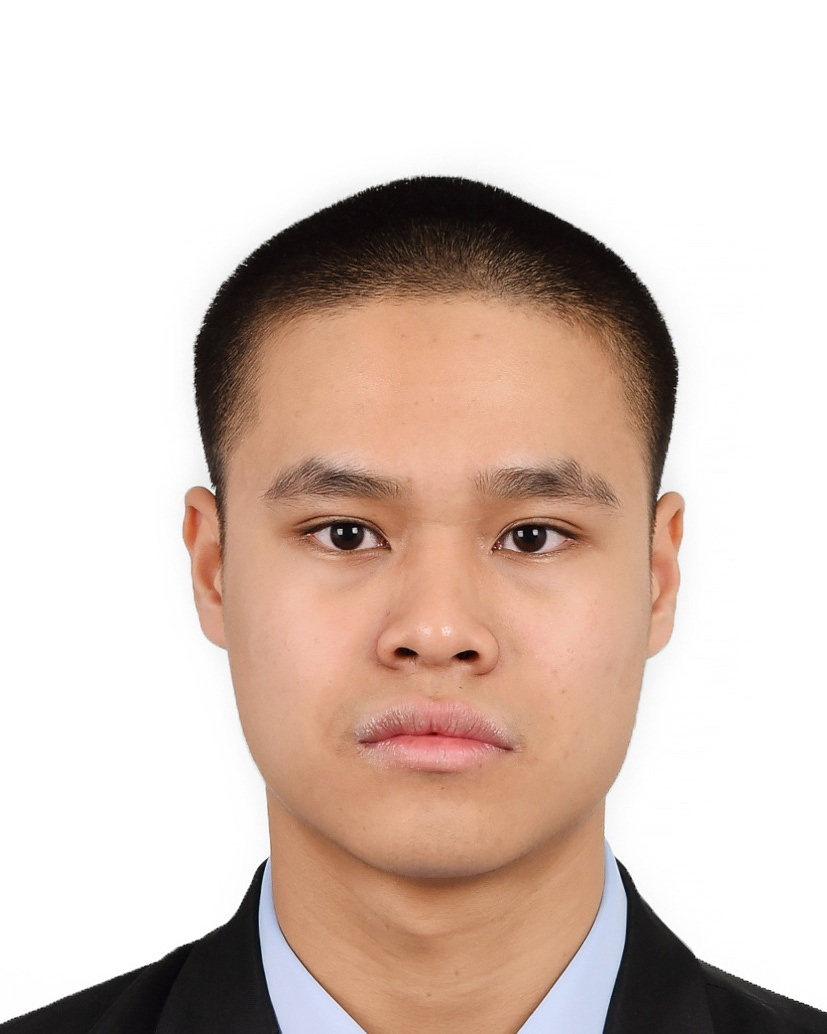
\includegraphics[width=1in,height=1.25in,keepaspectratio,clip]{figures/authors/wen-zer-goo.jpg}}]{Wen Zer Goo}
has undertaken diploma studies in information technology.

He is with the Research Centre for Human-Machine Collaboration (HUMAC), Faculty of Engineering and Technology, Sunway University, Bandar Sunway, Malaysia. His research focuses on visual obstacle perception and vision-language reasoning for simulated hexapod navigation. He has compared a task-trained YOLO detector, a pretrained YOLO-World detector, and a locally run vision-language model across seven obstacle scenarios, examining yielding, bypass behavior, and decision latency with a shared ROS 2 controller and RGB-D sensing.
\end{biography}

\begin{biography}[{
\includegraphics[width=1in,height=1.25in,keepaspectratio,clip]{figures/authors/anfel-fodil.jpg}}]{Anfel Fodil}
has undertaken diploma studies in computer science.

She is with the Research Centre for Human-Machine Collaboration (HUMAC), Faculty of Engineering and Technology, Sunway University, Bandar Sunway, Malaysia. Her research focuses on reinforcement learning and hexapod swimming. She combines proximal policy optimization with central pattern generators in NVIDIA Isaac simulations to study locomotion under mild water currents. She compares learned controllers with conventional central pattern generator baselines using swimming speed, stability, energy efficiency, and heading control.
\end{biography}

\begin{biography}[{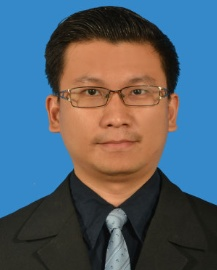
\includegraphics[width=1in,height=1.25in,keepaspectratio,clip]{figures/authors/tiong-yew-tang.jpg}}]{Tiong Yew Tang}
(Member, IEEE) received the bachelor's degree (Hons.) in information system engineering from Universiti Tunku Abdul Rahman in 2006 and the Ph.D. degree in information technology from Monash University in 2016.

He serves on the research committee at Sunway University, Malaysia. He is named as an inventor on a published international patent application filed under the Patent Cooperation Treaty. He works on applications of artificial intelligence in business research. His research interests include bibliometric analysis, artificial intelligence, deep learning, robotic process automation, business intelligence, big data analytics, and computational intelligence.

Dr. Tang received the Book Price Award in 2006 and the Dean's List Award in 2004 and 2005 from Universiti Tunku Abdul Rahman. In 2011, he received the PVC's Award for Excellence in Research, Teaching, and Administration (Round 2) from Monash University.
\end{biography}

\begin{biography}[{
\includegraphics[width=1in,height=1.25in,keepaspectratio,clip]{figures/authors/mohammad-ahmed-alomari.jpg}}]{Mohammad Ahmed Alomari}
(Senior Member, IEEE) received the M.Sc. and Ph.D. degrees in computer systems engineering from Universiti Putra Malaysia, Malaysia.

He is a Senior Lecturer with the Department of Cyber Security, Faculty of Artificial Intelligence and Cyber Security, Universiti Teknikal Malaysia Melaka, Melaka, Malaysia. He has authored and coauthored journal and conference papers. His research interests include mobile data storage encryption, security for smart grids and renewable energy systems, embedded systems, and cryptography. His current work also covers the Internet of Things, blockchain, and cloud computing.

Dr. Alomari is a Professional Technologist registered with the Malaysia Board of Technologists and a member of the International Association of Engineers. He reviews for Springer and SAI journals and serves on organizing and technical committees for conferences and workshops in Malaysia and Japan.
\end{biography}

\begin{biography}[{
\includegraphics[width=1in,height=1.25in,keepaspectratio,clip]{figures/authors/muhammad-hafidz-fazli-bin-md-fauadi.jpg}}]{Muhammad Hafidz Fazli Bin Md Fauadi}
received the bachelor's degree in industrial computing from Universiti Kebangsaan Malaysia in 2004, the M.Eng. degree in mechanical engineering (advanced manufacturing technology) from Universiti Teknologi Malaysia in 2006, and the D.Eng. degree in information, production, and system engineering from Waseda University, Japan, in 2012.

He is a Professor and the founding Dean of the Faculty of Artificial Intelligence and Cyber Security, Universiti Teknikal Malaysia Melaka, Melaka, Malaysia. His research interests include applied artificial intelligence, system simulation and optimization, intelligent manufacturing systems, cloud manufacturing, and the Internet of Things.

Prof. Muhammad Hafidz Fazli is a Certified HRDF Trainer, a Professional Technologist, and the Chief Editor of the \emph{Journal of Advanced Manufacturing Technology}.
\end{biography}

\endgroup
\EOD

\end{document}
